% Compile with pdflatex. The editable figure is included below.
\documentclass[11pt,letterpaper]{article}
\usepackage[T1]{fontenc}
\usepackage[utf8]{inputenc}
\usepackage{lmodern,microtype,tikz,hyperref,fancyhdr}
\usepackage[margin=0.88in,headheight=14pt,headsep=12pt]{geometry}
\usepackage[compact]{titlesec}
\definecolor{ink}{HTML}{1C4448}
\definecolor{steel}{HTML}{CBDCDA}
\definecolor{accent}{HTML}{883948}
\hypersetup{colorlinks=true,urlcolor=ink,linkcolor=ink}
\titleformat{\section}{\sffamily\Large\bfseries\color{ink}}{}{0pt}{}
\titleformat{\subsection}{\sffamily\normalsize\bfseries\color{ink}}{}{0pt}{}
\setlength{\parindent}{0pt}
\setlength{\parskip}{0.54em}
\setlength{\emergencystretch}{1.5em}
\pagestyle{fancy}\fancyhf{}\lhead{\small\sffamily NSF AMDO}\rhead{\small\sffamily Initial project description}\rfoot{\small\sffamily Collaborative working draft\quad\thepage}
\begin{document}

\section*{When to Blend Recycled Polypropylene Lots}

A compounder has two lots of recycled polypropylene and two orders due. A molded snap clip must flex far enough to engage its mating part. A ribbed housing must resist deflection and fill its thin ribs. Mixing the lots might supply both orders from one batch. It could also turn a lot suitable for clips into a blend that fails the clip requirement. Once the pellets are compounded together, the operator has lost the option to assign the original lots separately. We ask when testing a few grams of the proposed blend before committing the lots changes which orders can be filled.

\subsection*{Objective and intellectual merit}

We hypothesize that some pairs of lots produce a blend whose ductility departs reproducibly from the value predicted from the constituent lots. A small trial blend should be valuable when that departure crosses an order limit and a different routing is feasible. An equally plausible explanation is that the observed departure comes from sampling a heterogeneous sack or adding another melt-processing step. In that case extra measurements of the individual lots could buy as much useful information. We will test these explanations under equal assay budgets.

\begin{center}
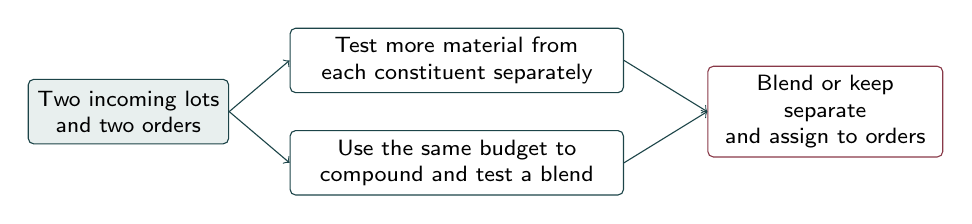
\begin{tikzpicture}[x=1cm,y=1cm,font=\sffamily\footnotesize,
 input/.style={draw=ink,fill=steel!45,rounded corners=2pt,align=center,minimum width=2.15cm,minimum height=.82cm},
 route/.style={draw=ink,rounded corners=2pt,align=center,text width=4.0cm,minimum height=.80cm},
 terminal/.style={draw=accent,rounded corners=2pt,align=center,text width=2.75cm,minimum height=.90cm}]
\node[input] (lot) at (0,0) {Two incoming lots\\and two orders};
\node[route] (single) at (4.17,.65) {Test more material from\\each constituent separately};
\node[route] (pair) at (4.17,-.65) {Use the same budget to\\compound and test a blend};
\node[terminal] (action) at (8.85,0) {Blend or keep separate\\and assign to orders};
\draw[ink,->] (lot.east) -- (single.west);
\draw[ink,->] (lot.east) -- (pair.west);
\draw[ink,->] (single.east) -- (action.west);
\draw[ink,->] (pair.east) -- (action.west);
\end{tikzpicture}
\end{center}

{\small\textbf{Figure 1.} Both assay strategies begin with the same routine lot records. The experimental comparison asks which additional test, performed before the lots are mixed, leads to more conforming material delivered to the two orders.}

Ten industrial batches bought to common melt-flow and density specifications exhibited elongations at break from about 10\% to 100\% [1]. A separate investigation of eleven recycled feedstocks identified interacting polymer phases as a source of mechanical variability [2]. Both studies establish differences among lots. Teruel and colleagues went further, using a recycler's records to predict flow, ash, impact strength and shrinkage for mixtures and to select input batches [3]. The missing evidence is whether physically assaying a proposed pair before choosing its route improves the decision beyond such a model and better sampling of its constituents.

For example, suppose equal quantities of lots A and B could separately fill a clip order and a housing order. The model predicts a common blend will fill both orders with one changeover saved. If a trial blend cracks during clip engagement, keeping A for clips and B for housings can protect the first order. If B also fails the housing test, the same warning need not make segregation worthwhile. The value of the test depends on the alternative assignment available that day.

The three-year project will establish the size and origin of blend departures, locate the order conditions where a trial blend could change routing, and test the value of that choice on independently processed material from unseen lots.

\newpage

\section*{Aim 1 · Separate a blend effect from sampling and processing history}

\textbf{Year 1.} Satish T. S. Bukkapatnam will lead the physical experiments. The first requirement is a compounder or molder willing to identify two orders, their demand, the allowable blend fractions and the actual acceptance tests. For the clip example we will measure the deformation at which a clip cracks and the force needed to engage it. For the housing we will measure stiffness and filling of the limiting feature. The owner must specify any required impact, shrinkage, dimensional or processing limits. Standard tensile bars can reveal a ductility change while the tooling is being arranged. The owner must establish how to accept material for each order before we can count kilograms qualified for it.

\subsection*{Construct the contrast}

We will retain portions of each source lot and draw material from multiple identified locations. In each production block we will prepare the two individual materials and one interior blend fraction permitted for both orders. Each pure material will undergo the same nominal compounding and molding histories as the mixture. We will record actual melt temperature, screw settings, residence time, molding conditions and specimen conditioning. This control matters because the extra melt pass or a change in thermal exposure can itself alter fracture behavior. In a separate comparison we will mold individual materials as received to estimate the effect of the additional processing pass.

A charge is a fresh weighing, mixing and compounding operation. Several bars molded from the same charge improve measurement precision. Repeated charges, independently drawn across sacks or defined within-lot locations, establish manufacturing repeatability. We will randomize run order within day, document machine cleaning and check carryover where the material changes. Xianyang Zhang will use the resulting lot, charge and specimen variation to size the independent trials for an order-relevant difference. Rui Tuo will choose overlapping pairs so that each training lot meets several partners. A repeatable response unique to a pairing is distinguishable from a consistently weak constituent only if a lot is tested with more than one partner.

\subsection*{Distinguish a physical effect from a change in the preferred route}

At a fixed blend fraction, we will compare the measured response with constituent-based mixing rules calibrated on separate training charges. Differential scanning calorimetry, melt-flow measurements and fracture-surface inspection on selected pairs can distinguish changes in crystallinity, composition and local failure morphology. We will measure melt flow or shear viscosity over the molding range and record evidence of incomplete fill. A mechanically promising blend that cannot be molded under the order's process limits cannot be assigned there. The first milestone is a reproducible departure large enough to change a feasible assignment. If individual-lot variation or thermal history accounts for it, training a richer pair model has little justification.

\newpage

\section*{Aim 2 · Decide which pairs warrant a trial blend}

\textbf{Year 2.} Tuo will model the constituent contribution to each property and the remaining dependence on the pair and blend fraction. Competing models will include a calibrated mixing rule and a batch-management predictor following Teruel et al. [3]. We will fit and tune the latter on the same training information as the proposed method and adapt its outcome set to the local specifications. Its historical commercial training data may be unavailable. The comparison will identify the predictors and properties that could be implemented locally.

The action is an allocation of finite stock. A solution specifies which masses to keep separate or blend at permitted ratios and assigns each resulting batch to an order, subject to demand and the qualifying tests. Tuo will target a small blend where the models disagree about an allocation. Zhang will carry uncertainty from new source lots and independent charges into each property's distance from its order limit. Local simulation checks provide a starting point for testing such discrepancies [4]. If all plausible estimates lead to the same allocation, running the small blend can only consume available material and time.

\subsection*{Give the competing assay its best use}

Both policies receive the same incoming records and routine tests. The constituent policy can spend its extra allowance on independent samples from the more uncertain lot or on a missing flow or mechanical test. The trial-blend policy can spend the allowance on compounding and measuring a small mixture or decline the test. We will fit the best constituent-only allocation rule, the published-model adaptation and the blend policy before final validation. Each will face the same caps on grams, staffed instrument time and deadline, with changeovers and conditioning charged. A no-extra-test policy will quantify the cost of purchasing information. We will separately report where the published-model adaptation makes the same correct routing choice.

\section*{Aim 3 · Fill the same orders from unseen lot pairs}

\textbf{Year 3.} Both source lots in every test pair will be absent from fitting, feature selection and threshold calibration. For the primary evaluation, test pairs will also use mutually disjoint source lots. We will reserve random portions of each lot before testing. Each policy receives an equivalent inventory and the same two orders, and records its allocation before the reserved stocks are processed. Independent outcome charges drawn from those stocks will implement each selected route, including separate processing when recommended. An inspector blinded to the recommendation will apply the same order-specific acceptance procedures, with the same sampling effort. For a subset selected before larger-scale results are seen, a processor will make the same pure and blended recipes on its line. We will compare mixing and cooling histories, flow behavior and order-specific failure modes across scales. A reversal in the preferred route at production scale will count as a failed transfer. Agreement at bench scale alone supports a conclusion about that scale.

\newpage

\section*{What constitutes a better manufacturing decision?}

For each held-out pair we will report the independently qualified mass delivered to the clip order and to the housing order, each capped at its demand. A kilogram may satisfy both specifications but can be delivered only once. We will debit material consumed by each policy's assays from its available inventory before allocation. We will also report unfilled demand by order, rejected mass, unassigned inventory, sample and changeover losses, and staffed time. The owner will declare priorities or shortage costs before seeing test-pair results. If additional housing mass comes at the cost of unfilled clips, that trade will remain visible. A whole-pair comparison and its uncertainty interval will preserve the independent unit of evidence. Replicate charges measure uncertainty in achieving the selected route. Repeated test bars cannot substitute for additional source lots.

\subsection*{Feasibility, team integration and scope}

The Texas A\&M Soft Matter Facility lists a microcompounder, piston injection molder, tensile tester and calorimeter [5]. Before budgeting, Bukkapatnam will seek traceable lots, operator time and fixtures. The first pilot will establish the mass needed for representative sampling and the repeatability of separately compounded charges. Tuo and Zhang will use that evidence jointly to fix allowable assay budgets, order-relevant margins and the number of independently sourced pairs. For the larger-scale check we need a processor, available batch mass and an agreed performance test on a molded feature. Without that access the deliverable is a laboratory decision experiment with explicit scale limits.

NSF's Convergence Accelerator has already funded work on selecting compatibilizers for variable recycled polypropylene, including predictive control of cost and quality [6]. Here the formulation additives are fixed. The proposed investment buys independently replicated comparisons of policies for testing and allocating real lots. The team will verify existing award deliverables, supplier and testing rights, facility commitments and an order owner's acceptance rules before requesting funds. If affordable constituent tests consistently match the trial blend, the output will identify when a compounder can omit that test.

\subsection*{Broader impacts}

We will develop a teaching exercise with lot assays, processing records, two orders and concealed independent test outcomes. Students and manufacturing trainees will allocate stock under a test budget before and after instruction using distinct lot pairs. We will match the difficulty of the two exercises using independent reference outcomes. We will measure qualified mass delivered to each order and material consumed by testing, comparing performance with an implementable fixed rule. A release of laboratory-generated records will include charge identifiers, failed batches and the assumptions needed to apply the exercise beyond the training materials.

\subsection*{Selected sources}

\begin{enumerate}
\small\setlength{\itemsep}{0pt}
\item \href{https://doi.org/10.1002/app.70501}{Impact of Seasonal Composition on the Long-Term Performance of Post-Consumer Recycled Polypropylene. Journal of Applied Polymer Science, 2026.}
\item \href{https://doi.org/10.1016/j.wasman.2026.115586}{Kianpisheh et al. Identifying the roots of property variability in recycled polypropylene. 2026.}
\item \href{https://doi.org/10.1016/j.jclepro.2023.140390}{Teruel et al. Machine learning and input batch management for recycled polypropylene. 2024.}
\item \href{https://arxiv.org/abs/2604.17144}{Li, Zhang and Tuo. Statistical validation of computer models. Preprint, 2026.}
\item \href{https://somf.engr.tamu.edu/instruments/}{Texas A\&M University. Soft Matter Facility instrument inventory.}
\item \href{https://nsf-gov-resources.nsf.gov/2022-12/2022%20Cohort%20Track%20I%20Phase%201%20Award%20Announcements%20-%20Black%20%26%20Decker%20%28u.s.%29%20Inc.508.pdf}{NSF. Economically Sustainable Polypropylene Recycled Plastics Enabled by Compatibilizer Additives. Convergence Accelerator contract 49100423C0004.}
\end{enumerate}
\end{document}
